\documentclass[11pt,a4paper]{article}
\usepackage[a4paper, hmargin={2.5cm,2.5cm},vmargin={2.5cm,2.5cm}]{geometry}
\usepackage{graphicx}
\usepackage{cmap}
\usepackage[utf8]{inputenc}
\usepackage[english]{babel}
\usepackage{amsmath}
\usepackage{amsfonts}
\usepackage{listings}
\usepackage{color}
\usepackage{pdfpages}
\usepackage{fancyvrb}
\usepackage{fancyhdr}
\usepackage{lipsum}
% \usepackage{pgfplots}
\usepackage{wrapfig}
\usepackage{mathtools}
\usepackage{subfig}
\usepackage{enumitem}
\usepackage{tikz}
\usepackage{forest}
\usepackage{fancyvrb}
\usepackage{pdflscape}
\usepackage{mathpartir}
\usetikzlibrary{automata, positioning, arrows}
\usetikzlibrary{positioning}
\usetikzlibrary{shapes,shapes.geometric,arrows,fit,calc}


\usetikzlibrary{automata, positioning, arrows}
\usetikzlibrary{positioning}
\usetikzlibrary{shapes,shapes.geometric,arrows,fit,calc}

\def\dunderline#1{\underline{\underline{#1}}}
\def\indent{\space\space\space\space}

\begin{document}
\begin{titlepage}
  \title{Programmer som data trial exam}
  \author{Albert Ross Johannessen}
  \maketitle
  \newpage
  \thispagestyle{empty}
  \newpage
\end{titlepage}

\pagestyle{fancy}
\fancyhf{}
\rhead{Programmer som data}
\rfoot{Page \thepage}
\newpage
%\begin{landscape}
%\end{landscape}
\section{Opgave 1}
Betragt den ikke-deterministiske endelige automat (''nondeterministic finite automaton'', NFA) nedenfor. Det anvendte alfabet er $\{\text{\Verb|a,b|}\}$. Der er i alt 5 tilstande, hvor 5 er den eneste accetptilstand.
\begin{figure}[!ht]\label{fig:examfignfa}
  \centering
  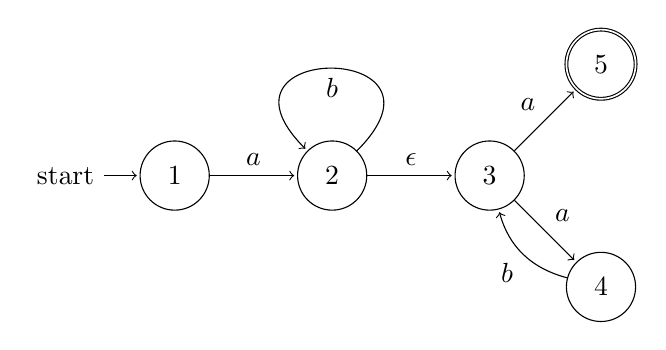
\begin{tikzpicture}[shorten >=1pt,node distance=2cm,on grid,auto] 
     \node[state, initial] (s_1)   {$1$}; 
      \node[state] (s_2) [right =of s_1] {$2$};
      \node[state] (s_3) [right =of s_2] {$3$};
      \node[state] (s_4) [below right =of s_3] {$4$};
      \node[state, accepting] (s_5) [above right =of s_3] {$5$};
            
      \path[->] 
      (s_1) edge  node {$a$} (s_2)
      (s_2) edge [loop] node {$b$} (s_2)
      (s_2) edge  node {$\epsilon$} (s_3)
      (s_3) edge  node {$a$} (s_5)
      (s_3) edge  node {$a$} (s_4)
      (s_4) edge [bend left] node {$b$} (s_3)
      ;
  \end{tikzpicture}
  \caption{The labeled NFA}
\end{figure}
\subsection{Angiv all årsager til at automaten er ikke-deterministisk}
\begin{enumerate}
  \item Der går en epsilon kant fra 2 til 3.
  \item Der går 2 $a$ kanter fra 3.
\end{enumerate}
\subsection{Giv tre eksempler på strenge der genkendes af automaten}
\begin{enumerate}
  \item aa
  \item abbba
  \item ababa
\end{enumerate}
\subsection{Giv en uformel beskrivelse af sproget (mængden af alle strenge) der beskrives af automate}
Sproget der beskrives af automaten har følgende regler.
\begin{itemize}
  \item Strenge skal starte og slutte på a
  \item Det første a kan være efterfulgt af et vilkårligt antal b'er
  \item I den efterfølgende streng, hvis man vil have mere end ét a så skal alle a'er være sepereret af b'er
\end{itemize}
\newpage
\subsection{Konstruer den tilsvarende DFA}
\begin{figure}[!ht]\label{fig:nfa2dfa}
  \centering
  \begin{tabular}{c|ccc}
          & $a$ & $b$ & NFA State\\\hline
    $S_1$ & $\left\{2,3\right\}^{S_2}$ & $\left\{\right\}$ & $\left\{1\right\}$ \\
    $S_2$ & $\left\{4,5\right\}^{S_3}$ & $\left\{\right\}^{S_2}$ & $\left\{2,3\right\}$ \\
    $S_3$ & $\left\{\right\}$ & $\left\{3\right\}^{S_4}$ & $\left\{4,5\right\}$ \\
    $S_4$ & $\left\{4,5\right\}^{S_3}$ & $\left\{\right\}$ & $\left\{3\right\}$ \\
  \end{tabular}
\end{figure}
\begin{figure}[!ht]\label{fig:examfigdfa}
  \centering
  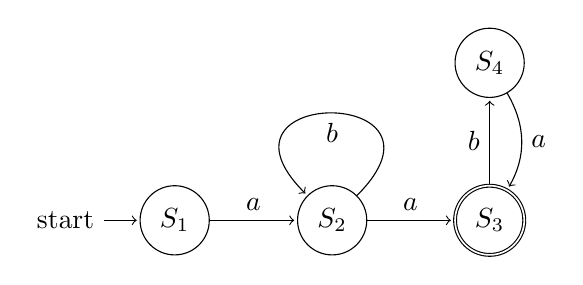
\begin{tikzpicture}[shorten >=1pt,node distance=2cm,on grid,auto] 
     \node[state, initial] (s_1)   {$S_1$}; 
      \node[state] (s_2) [right =of s_1] {$S_2$};
      \node[state, accepting] (s_3) [right =of s_2] {$S_3$};
      \node[state] (s_4) [above =of s_3] {$S_4$};
            
      \path[->] 
      (s_1) edge  node {$a$} (s_2)
      (s_2) edge [loop] node {$b$} (s_2)
      (s_2) edge  node {$a$} (s_3)
      (s_3) edge  node {$b$} (s_4)
      (s_4) edge [bend left] node {$a$} (s_3)
      ;
  \end{tikzpicture}
  \caption{The labeled NFA}
\end{figure}
\begin{figure}[!ht]\label{fig:g1}
  \centering
  \begin{tabular}{c|c}
    $G_1$ & $\left\{S_1,S_2,S_4\right\}$\\
    $G_2$ & $\left\{S_3\right\}$
  \end{tabular}
\end{figure}
\begin{figure}[!ht]\label{fig:testg1}
  \centering
  \begin{tabular}{c|cc}
    $G_1$ & $a$ & $b$\\\hline
    $S_1$ & $G_1$ & - \\
    $S_2$ & $G_2$ & $G_1$ \\
    $S_4$ & $G_2$ & -
  \end{tabular}
\end{figure}
\begin{figure}[!ht]\label{fig:g1}
  \centering
  \begin{tabular}{c|c}
    $G_2$ & $\left\{S_3\right\}$\\
    $G_3$ & $\left\{S_1\right\}$\\
    $G_4$ & $\left\{S_2\right\}$\\
    $G_5$ & $\left\{S_4\right\}$\\
  \end{tabular}
\end{figure}
Siden der er én gruppe pr knude så er vores DFA så lille som den kan være.
\subsection{Angiv et regulært udtryk for automaten}
Hvis vi kigger på NFA'en som vi får givet i opgave beskrivelsen så kan vi splitte den op.
\begin{align*}
  1\xrightarrow{a}2 &= a\\
  2\xrightarrow{b}2 &= b*\\
  3\xrightarrow{a}4\xrightarrow{b}3 &= \left(ab\right)*\\
  3\xrightarrow{a}5 &= a
\end{align*}
Hvis vi sætter dem sammen får vi følgende udtryk.
\begin{align*}
  \text{\Verb|ab*(ab)*a|}
\end{align*}
Det samme kan vi gør for DFA'en
\begin{align*}
  S_1\xrightarrow{a}S_2 &= a\\
  S_2\xrightarrow{b}S_2 &= b*\\
  S_2\xrightarrow{a}S_3 &= a\\
  S_3\xrightarrow{b}S_4\xrightarrow{a}S_3 &= \left(ba\right)*\\
\end{align*}
Hvilket producerer følgende udtryk.
\begin{align*}
  \text{\Verb|ab*a(ba)*|}
\end{align*}
Her er det indlysende at se at at det er det samme udtryk men skrevet på en anden måde, der er som udgangspunkt ikke nogen forskel mellem \Verb|a(ba)*| og \Verb|(ab)*a|.
\end{document}
